\documentclass[authordate, empirical]{jote-new-article}

\usepackage{caption}

\usepackage{tabularx}

\usepackage{graphicx}

\usepackage{hyperref}

\usepackage[backend=biber,style=apa]{biblatex}

\addbibresource{bibliography.bib}

\jotetitle{The Impact of Incentivization on Recruitment, Retention, Data Quality, and Participant Characteristics in Ecological Momentary Assessments}
\keywordsabstract{ambulatory assessment, experience sampling, compensation, research participation effects, mood}
\abstracttext{Ecological Momentary Assessment (EMA) study participation is usually incentivized using monetary (e.g., fixed or performance-contingent payment) or non-monetary (e.g., feedback) compensation. This study investigates the impact of this incentivization on recruitment, retention, data quality, and participant characteristics in a sample of 74 students. For this purpose, an EMA study (time-based sampling) was conducted in participants’ daily life using a 2 Payment (fixed/ performance-contingent) x 2 Feedback (yes/ no) experimental between-subjects design. Offering feedback increased the likelihood of participation and reduced the likelihood of participants receiving fixed payment to drop out. Offering feedback additionally improved data quality. Furthermore, offering feedback attracted participants with higher interest in research and the study topic. Offering fixed vs performance-contingent payment had little effect on the outcomes of interest. Offering feedback as compensation in EMA studies may facilitate recruitment and increase data quality; however, it may also risk higher selection bias. Conclusions are drawn from a relatively small student sample; the results thus need to be replicated in larger and more diverse samples.}
\runningauthor{Giese et al.}
\jname{Journal of Trial \& Error}
\jyear{2024}
\paperdoi{10.36850/28b4-4f59}
\paperreceived{November 13, 2023}
\author[1,2]{\mbox{Helge Giese\orcid{0000-0001-7609-0215}}}
\affil[1]{Department of Psychology, University of Konstanz}
\affil[2]{Heisenberg Chair for Medical Risk Literacy and Evidence-based Decisions, Center of Anestesiology and Intensive Care Medicine, Charité - Universitätsmedizin Berlin}
\corremail{\href{mailto:helge.giese@charite.de}{helge.giese@charite.de}}
\corraddress{Charité - Universitätsmedizin Berlin}
\runningauthor{Giese \& König}
\author[3,4]{\mbox{Laura M König\orcid{0000-0003-3655-8842}}}
\affil[3]{Faculty of Life Sciences: Food, Nutrition and Health, University of Bayreuth}
\affil[4]{Faculty of Psychology, University of Vienna}
\paperaccepted{September 27, 2024}
\paperpublished{November 16, 2024}
\paperpublisheddate{2024-11-16}
\jwebsite{https://journal.trialanderror.org}



\begin{document}
\begin{frontmatter}
  \maketitle
  \begin{abstract}
    \printabstracttext
  \end{abstract}
\end{frontmatter}









	







	\section{Introduction}



	Ecological Momentary Assessment (EMA), i.e., the repeated assessment of study participants in real-time and real-life, may help to overcome limitations of traditional self-report measures such as recall bias in questionnaires. It furthermore allows to study phenomena as they naturally occur in different contexts in daily life, and repeatedly over time, so increasing ecological validity compared to questionnaire or experimental laboratory studies (Shiffman et al., 2008). EMA is therefore increasingly used in research to investigate behaviors and their determinants (Perski et al., 2023), thereby contributing to the formulation and testing of theory (Scholz, 2019) and interventions (Berli et al., 2021).



	To draw meaningful conclusions from EMA data with sufficient certainty, large samples generating large numbers of responses are required (Bolger \& Laurenceau, 2013). EMA usually requires participants to complete several assessments per day over the course of one to several weeks (König, Van Emmenis, et al., 2022; Wrzus \& Neubauer, 2022), which may complicate recruitment and retention due to reduced willingness of taking part in or completing the study (Eisele et al., 2022). Furthermore, participants might miss prompts or events to record (Ziesemer et al., 2020), or respond carelessly (Eisele et al., 2022), which leads to reduced data quality.



	To overcome this challenge, researchers commonly offer monetary incentivization for EMA study participation (Ottenstein \& Werner, 2021; Wrzus \& Neubauer, 2022), which has previously been shown to improve response rates in several study designs (Edwards et al., 2009; Gillies et al., 2021; Keusch, 2015; Voslinsky \& Azar, 2021). Some EMA studies offer fixed payment, i.e., all participants receive the same amount of money irrespective of how many surveys or study days they completed; others offer performance-contingent payment, e.g., by offering a certain amount of money per answered prompt. Yet again other studies offer non-monetary incentives such as personalized feedback based on the collected data (Ottenstein \& Werner, 2021; Wrzus \& Neubauer, 2022).


	\begin{takeHomeMessage}
		Incentivization methods in EMA studies need to be carefully selected not only based on feasibility considerations and availability of funding, but also based on the potential impact on attrition, data quality, and certain participant characteristics. However, the current results need to be replicated in larger samples to test generalizability to more diverse samples and other study topics.
	
	\end{takeHomeMessage}

	A reason for non-monetary incentives beyond budget constraints is the hope of researchers that personalized feedback may improve recruitment and retention due to increased personal relevance and motivation (Pratap et al., 2020; van Gelder et al., 2018): If participants would like high quality feedback they have to participate conscientiously. However, providing personalized feedback might also increase recruitment bias, as it may especially appeal to people with a strong interest in the topic (Cheung et al., 2017). This may aggravate existing self-selection biases, as participants in behavioral research are healthier (Haynes \& Robinson, 2019), younger, wealthier, and more highly educated (Henrich et al., 2010; Pratap et al., 2020) than the population average, limiting both the generalizability and the potential impact of this research.



	Ottenstein and Werner (2021) compared the impact of incentivization on retention and data quality in EMA studies, indicating that performance-contingent monetary incentivization may increase compliance compared to fixed payment. However, they were unable to draw conclusions regarding differences between monetary and non-monetary incentives since the number of studies reporting to have offered non-monetary incentives was small. Even more importantly, incentivization schemes could only be compared across studies since direct experimental comparisons are rare (Ottenstein \& Werner, 2021; Wrzus \& Neubauer, 2022). Studies that include at least quasi-experimental incentive conditions merely indicate that not providing any rewards harms EMA participation rates (Ludwigs et al., 2020) or that course credit is less valued than monetary or prize rewards (Harari et al., 2017).



	This study therefore aims to provide a comprehensive experimental test of fixed vs performance-contingent payment and additional provision of feedback as non-monetary incentivization on recruitment, retention, data quality (operationalized as internal consistency per participant), and participant characteristics in an EMA study. We expected monetary incentivization to impact recruitment, retention, and data quality through fixed payments. Specifically, we expected fixed payment to yield more participants initially recruited (compared to performance-contingent payment) since the outlook to receiving a fixed payment is more attractive (due to higher attractiveness of the reward; H1). At the same time, we expected fixed payment (vs. performance-contingent payment) to lead to more drop-outs (i.e. participants not recording data until the last day) since, in this condition, payment is certain independently of the performance (H2). Based on the same reasoning, we expected fixed payment to yield fewer prompts being answered compared to performance-contingent payment (H3). Finally, we expected fixed payment to yield better data quality compared to performance-contingent payment, as indicated by the internal consistency of the scales (H4). This is because participants might be more intrinsically motivated to provide a response if they receive the same amount of money independent of whether they respond to the prompt or not, while performance-contingent payment might induce speeding to make sure that the prompt, and thus the payment, will not be missed.



	Furthermore, we expected feedback provision to impact recruitment, retention and participant characteristics. Specifically, we expected feedback provision to decrease drop-out (H5) and to increase data quality (H6) since the recorded data will become more meaningful to the individual with the promised feedback. We expected feedback provision to increase the number of people initially interested in the study (H7), but also to attract more participants with a stronger interest in the study topic (H8) since the feedback will allow them to learn about themselves. Finally, we also explored differences in demographic and psychological participant characteristics between groups.



	\section{Materials and methods}



	The study procedure and data analysis plan were preregistered prior to data collection (\href{https://osf.io/cwb3h/}{https://osf.io/cwb3h/}). Materials and data are available in the Open Science Framework (\href{https://osf.io/zbe5q/}{https://osf.io/zbe5q/}).



	\subsection{Sample}



	Participants were recruited from the online study pool of the University of Konstanz. All members of the pool (\emph{N} = 707 at the start of the study) were randomly assigned to one of four groups and only saw the corresponding study advertisement. Eligible participants had to be able to read and write German and own an Android smartphone to be able to use the study app. Based on previous studies for which participants were recruited via the study pool, recruiting 200 participants was deemed feasible. However, recruitment had to be halted in November 2021 before reaching that threshold due to limited availability of funding.



	\subsection{Study design}



	The study used a between-subjects design and time-based sampling. Data was collected between February and November 2021. The study adhered to the Declaration of Helsinki; general ethical approval was obtained from the University of Konstanz ethics committee.



	All members of the study pool were invited via email to take part in an EMA study about mood fluctuations. The study descriptions (see supplementary material) were identical for all conditions except the information about compensation. Participants were randomly assigned to one of the 2 \emph{Payment }(fixed/performance-contingent) x 2 \emph{Feedback }(yes/no) conditions. Participants in the fixed payment conditions received €15. Participants in the performance-contingent payment conditions received €1 for completing the online questionnaire and €0.20 per answered prompt (equaling to a maximum of €15 for perfect retention). All participants were able to convert money into course credit, with €5 amounting to 0.5 hours of course credit. Participants in the feedback condition additionally received printed feedback with visualizations depicting the fluctuations of their mood during the study period (see supplemental material for an example). Participants only received feedback after the study period to avoid influences on the mood data being collected (c.f. König, Allmeta, et al., 2022).



	\subsection{Procedure}



	Upon sign-up, participants filled in an online questionnaire. They provided informed consent by ticking a box on the first page. The questionnaire assessed basic demographic information and motivation for taking part in the study. At the end of the questionnaire, participants received instructions for how to install the study app (movisensXS, movisens GmbH, Karlsruhe) and a personalized QR code to download the study questionnaires on their phone. They were then asked to record their mood for 7 consecutive days by responding to 10 random prompts per day that were sent between 8:00 am and 9:00 pm, with at least 15 minutes between prompts. Each EMA prompt only contained the six items to assess mood, which took participants on average 20 seconds (median = 16 seconds) to complete. Afterwards, participants received instructions for how to uninstall the study app. To receive their payment and written feedback (if applicable), they met with a researcher at the university.



	Recruitment was initially started in January 2021, but due to pandemic-related restrictions, recruitment was slow. We therefore halted recruitment in February and continued in May 2021. Since recruitment was still slow due to ongoing restrictions, we halted recruitment again during the semester break (July to October) and recruited again in November 2021. Recruitment was then ended since the funding required for paying participants was no longer available.



	\section{Measures}



	\subsection{Mood}



	Participants' mood was assessed using the Wilhelm and Schoebi (2007) scale, which assesses valence (content/discontent; unwell/well), calmness (agitated/calm; relaxed/tense) and energetic arousal (tired/awake; full of energy/without energy) with two items each. Responses were indicated on seven-point semantic differentials. Internal consistencies per group are reported as part of the results.



	\subsection{Questionnaire data}



	\emph{Trust in science} was assessed with a three-item questionnaire from the German Wissenschaftsbarometer 2021 (Wissenschaft im Dialog/ Kantar, 2021). Responses were indicated on a 6-point scale from 1 - trust entirely to 5 - trust not at all (α = .42 in the entry questionnaire).



	\emph{Motivations for signing up for the study }were assessed with six items on a 5-point scale (1 - does not apply at all to 5 - fully applies). These items were evaluated separately, because they were meant to assess a specific reason each, namely: (1) personal interest in the topic; (2) to support research; (3) financial compensation; (4) to collect course credit; (5) participating in research studies is fun; (6) to learn more about myself.



	\emph{Motivation to complete the study }was assessed with one item (How motivated are you to complete the study?) on a 5-point scale (1 - not at all to 5 - very).



	\emph{Affinity to technology} (Franke et al., 2019) was assessed with the four-item short-form of the corresponding scale (Wessel et al., 2019). Responses were indicated on a 6-point scale from 1 - completely disagree to 6 - completely agree (α = .87 in the entry questionnaire).



	\emph{Big Five. }Basic personality traits according to the Big Five (Costa \& McCrae, 1992) were assessed with the 10-item short form of the Big Five Inventory (Rammstedt \& John, 2007;\emph{ r}\textsubscript{\emph{ext}} = .62;\emph{ r}\textsubscript{\emph{agr}} = .10; \emph{r}\textsubscript{\emph{con}} = .46;\emph{ r}\textsubscript{\emph{neu}} = .49;\emph{ r}\textsubscript{\emph{ope}} = .57 in the entry questionnaire).



	\emph{Demographic characteristics.} Age (“Your age”, followed by an open text field), gender (“You are …” followed by the response options male, female, diverse), and monthly net household income (using the following six categories and “not specified”: up to €500; €501 to €1,000; €1,001 to €1,500; €1,501 to €2,000; €2,001 to €2,500; €2,501 and more) were assessed.



	\section{Statistical analysis}



	\subsection{Preprocessing of EMA data}



	\emph{Recruitment success} was assessed by the proportion of participants enrolled per condition out of all invited members of the study pool at the start of the study. The speed of enrollment was determined by the rank of the day the participants completed the entry-questionnaire.



	\emph{Retention }was operationalized by a) the number of people completing the one-week EMA period (answering the 71st prompt) in relation to the number of invited and enrolled participants, and b) by the number of fully answered prompts. The drop-out speed was determined by the last prompt answered.



	\emph{Data quality. }Internal consistency of a six-item mood scale (Wilhelm \& Schoebi, 2007) was computed per participant. That is, all entries of an individual participant across time were considered separate entries, and Cronbach's alpha was computed for each participant based on all EMA entries on the mood scale. In the context of this study, this measure is regarded as an indicator of high data quality of a participant and not used as a measure of scale reliability.



	\subsection{Statistical models}



	As pre-registered, we effect-coded the two between-factors and used logistic regressions for binary outcomes (recruitment success and drop-outs), cox regressions for analyses for speed of recruitment and drop-out, and ANOVAs for continuous outcomes. We decided against pre-registered MANOVAs for continuous outcomes, since it was not clear which outcomes should be summarized in them. Because the sample size was much lower than expected in the pre-registration, we decided not only to report significant results with \emph{p} < .05, but also marginally significant results with \emph{p} < .10, for which we do not want to dismiss an effect in acknowledgement of the limited achieved power. Significant and marginally significant interactions were thus followed by simple-effect analyses.



	The pre-registered strategy to determine drop-out speed was ambiguous as to whether the days of the last prompt should be used as a speed indicator and how participants not providing any EMA data should be handled. We opted for the last successful prompt analyses, also because with the day criterion, only seven people were considered dropping out early (1 after 4 days, and 3 on day 5 and 6). Regarding the handling of participants not providing EMA data, we opted to report test statistics excluding them, but also present data on statistics including them, where feasible.



	\section{Results}



	\subsection{Sample description}



	A total of 88 participants started the entry questionnaire, 14 of which did not indicate an identifier or were double entries caused by linking difficulties and entry errors and were therefore discarded. The final sample for analyses regarding motivation and study participation thus consisted of 74 (86\% female; \emph{M}\textsubscript{age}\emph{ }= 23.29, \emph{SD }= 4.97 years; \emph{n}\textsubscript{fixed and feedback }= 21, \emph{n}\textsubscript{fixed and no feedback }= 14, \emph{n}\textsubscript{performance-contingent and feedback }= 24, \emph{n}\textsubscript{performance-contingent}\textsubscript{ and no feedback }= 15) of the 707 eligible members of the study pool. Out of these individuals, 70 could successfully be linked to entries in the study app. The other four did not provide a matching identification code in the EMA questionnaire. From these 70 entries, one did not provide data in the app except the identification code, leaving 69 participants in the EMA dataset to be analyzed. On average, participants responded to 40.7 out of the 70 mood prompts, yielding a compliance rate of 58\%.



	\subsection{Does the incentivization influence study participation and recruitment speed?}



	Overall, participants that were offered \emph{feedback} were marginally more likely to participate (\emph{B} = 0.48, \emph{OR} = 1.62, 95\% CI(0.99; 2.65), \emph{p} = 0.056, 45/355 vs. 29/352) in the study. Similarly, these participants signed up for the study at a marginally higher rate across time by completing the entry questionnaire (\emph{B} = --0.45, \emph{HR} = 0.64 95\% CI(0.40; 1.01), \emph{p} = 0.057; see also Figure S1 in the supplementary material); this can be seen as initial evidence for H7. Both \emph{payment} and the payment x feedback interaction played no discernible role in participation decisions (all |\emph{B}| ≤ 0.11; all \emph{p} ≥ 0.816); H1 was thus rejected.



	\subsection{Does the incentivization influence retention?}



	Considering completed EMA questionnaires, there was only a numerical, but no significant advantage for incentivization conditions including feedback (17/355 vs. 9/352, \emph{p} = 0.103). When only considering all individuals that finished the entry questionnaire (\emph{N} = 74), the recruitment strategies generally had no discernible effect on the number of successful EMA entries (all \emph{F}(1, 70) < 1.21, \emph{p} ≥ 0.275, η²\textsubscript{p} ≤ 0.017), or whether the final prompt was answered (all \emph{p} ≥ 0.212). Both H2 and H5 thus had to be rejected. However, when only considering the 69 individuals that actually provided EMA data, the rate of dropout determined by the final prompt answered was marginally affected by an unexpected \emph{payment x feedback }interaction (\emph{B} = 1.23, \emph{HR} = 3.41 95\%CI(1.00; 11.63), \emph{p} = 0.050; see also Figure S2 in the supplementary material): In the fixed payment group, participants without feedback dropped out at a higher rate than with feedback (\emph{B }= --0.92, \emph{HR} = 0.40 95\%CI(0.17; 0.95), \emph{p} = 0.037), while no differences emerged for the performance-contingent payment groups based on feedback (\emph{B} = 0.31, \emph{HR} = 1.37 95\%CI(0.57; 3.26), \emph{p} = 0.484). Regarding the number of successfully answered prompts, participants with a performance-contingent payment scheme answered marginally more prompts (\emph{M }= 46.19, \emph{SD }= 14.35) compared to the fixed payment scheme (\emph{M }= 40.85, \emph{SD }= 14.52; \emph{F}(1, 65) = 3.00, \emph{p} = 0.088, η²\textsubscript{p} = 0.044). This can be seen as initial evidence for H3.



	\subsection{Does the incentivization influence EMA data quality?}



	While most of the 69 participants with EMA data missed the reverse-coding of mood items in the EMA questionnaire and therefore had negative internal consistencies, both feedback (\emph{M }= --1.79, \emph{SD }= 1.27 vs \emph{M }= --2.76, \emph{SD }= 2.06; \emph{F}(1, 65) = 6.38, \emph{p} = 0.014, η²\textsubscript{p} = 0.089) and marginally also fixed payment (\emph{M }= --1.80, \emph{SD }= 1.36 vs \emph{M }= --2.53, \emph{SD }= 1.90, \emph{F}(1, 65) = 3.67, \emph{p} = 0.060, η²\textsubscript{p} = 0.054) led to higher values indicating potentially higher -- but still completely unreliable -- data quality. H6 was thus confirmed. There is also some initial evidence for H4, although the hypothesis had to be formally rejected since the analysis fell short of reaching the predetermined threshold for statistical significance.



	\subsection{Does the incentivization influence participation motivation and sample characteristics?}



	Results are summarized in Table 1 and Figure 1. Overall, participants indicated higher motivation to complete the study in the fixed compared to the performance-contingent payment condition. Furthermore, there was a marginally significant effect of payment with fixed payment yielding participants with somewhat higher epistemic interest, while feedback recruited people with both more epistemic interest and personal interest in the topic of the study; H8 was thus confirmed. The interest to support science was marginally lower in the performance-contingent payment groups when no additional feedback was provided. The marginal \emph{payment x feedback }effect in trust in science additionally indicates that people with the no feedback, performance-contingent payment scheme were specifically more trusting in science than the other conditions.



	Concerning general demographics, there was no difference by incentivization scheme, except that participants in the fixed payment scheme were more neurotic. Trait openness was specifically low for fixed payment incentivization with feedback.



	\section{Discussion}



	This study experimentally tested the impact of monetary and non-monetary incentivization on recruitment, retention, data quality, and participant characteristics in an EMA study. Monetary and non-monetary incentives differentially affected the outcomes of interest, indicating that careful considerations need to be made regarding incentivization to reach specific goals, e.g., regarding recruitment speed or diversity of the sample.



	\subsection{Implications for recruitment}



	It was assumed that providing fixed payment would yield more participants recruited (H1), but this hypothesis could not be confirmed. Results provide some evidence for the assumption that offering performance-contingent payment would lead to more prompts being answered (c.f., H3). This confirms the notion derived from comparing studies with different incentivization schemes in Ottenstein and Werner (2021) that performance-contingent payment might be advantageous over fixed payment, at least when it comes to the amount of data that can be collected per participant. At the same time, results provide a first indication that offering feedback may facilitate recruitment both regarding the total number of participants (c.f., H7) and the recruitment speed, with small to medium effect sizes. However, the effect fell short of reaching the threshold for statistical significance specified in the preregistration; replications are required to confirm the findings.



	\subsection{Implications for retention}



	Furthermore, it was expected that fixed payment would lead to more drop-out (H2) and that feedback provision would decrease dropout (H5). Indeed, fixed payment even led to higher drop-out rates when no additional incentive for answering prompts was provided by offering feedback. This points towards a potential buffering role of feedback, which may sustain interest in the study and willingness to record — a pattern similarly found in studies showing higher engagement with self-monitoring in interventions with feedback (Burke et al., 2011). Thus, if a provision of performance-contingent payment is not possible, e.g., because of a lacking ground truth as in event-contingent dietary EMA studies (König, Van Emmenis, et al., 2022; Ziesemer et al., 2020), offering feedback may be crucial in retaining participants. Yet, this suggestion is somewhat speculative since the present study did not include a “feedback only” condition, which should be explored in future research.



	\subsection{Implications for the sample composition}



	The implications for sample composition are especially important since potential benefits of providing feedback for participant recruitment may come at the cost of increasing selective sampling of participants as indicated by higher intrinsic motivation and interest of participants signing up for the study in feedback conditions (c.f., H8). Similar issues also occur when offering a fixed payment scheme irrespective of answered prompts. This selectivity may be particularly problematic in studies which aim to generalize effects to a population. Therefore, feedback and fixed payment schemes may impair efforts to recruit populations that are more difficult to reach. Since motivations to take part in the study were only assessed after and not prior to assignment to a condition, the present study cannot rule out that the condition might also have influenced motivation. Future studies should therefore tap into the underlying psychological mechanisms of study incentivization to shed further light on this issue.



	Furthermore, one should also take into account that these two incentivization strategies may increase self-selection biases hampering study conclusions up to the point of misjudging e.g. predictor-outcome relationships or the effect of an intervention (Biele et al., 2019; Humphreys et al., 2014; see also Bethlehem, 2010). Thus, active self-selection needs to be carefully considered as a potentially negative consequence of offering feedback as a low-cost alternative incentivization. On the other hand, the potential prerequisite of higher trust when solely receiving performance-contingent payment (as a sign of trust in the scientist to fairly evaluate the performance) may also decrease generalizability when only relying on this incentivization method, especially because trust in science is an important predictor of belief in misinformation (e.g., Agley \& Xiao, 2021) and even adherence to health-protective measures (Devine et al., 2021).



	The present study did not find meaningful differences between groups regarding sociodemographic characteristics. This is potentially due to the homogeneous study pool used for recruitment, which mainly consisted of students who take part in studies in exchange for course credit. This also raises potential ethical concerns regarding incentivization of study participation; ethics committees are usually concerned with potential undue influence due to excessive payment, which may undermine consent and encourage participants to take risks that they would not accept without payment (see e.g., Gelinas et al., 2018 , for a discussion). In the context of the present study, we adhered to regulations of payment set by the study pool; in other contexts, researchers may need to carefully weigh payment thresholds and their potential influence on participants (Dickert et al., 2002). At the same time, some form of payment may only seem fair, given that participants volunteer their time which they could otherwise spend working a paid job (Bierer et al., 2021). This is especially true for participants with low socio-economic status which are often underrepresented in research (Krukowski et al., 2024). The research community thus should continue the debate on payment practices, taking not only feasibility and research outputs, but also ethical considerations into account.



	\subsection{Implications for data quality}



	As a potential positive consequence, the sampling of more highly motivated participants in feedback and fixed payment schemes may also increase data quality. A first, speculative indication of this may be seen in the effects the experimental condition had on internal consistency of individual responses for both fixed payment (c.f., H4) and feedback provision (c.f., H6). Thus, deciding against offering feedback or fixed payment to diversify the sample may impose potential costs in data quality. Because the internal consistencies were negative and responses of a single person violate the independence assumption, these results should be confirmed by other means such as the compliance to potential attention checks.

	\begin{originalPurpose}




		Recent reviews stated that the method chosen to incentivize participation in Ecological Momentary Assessment (EMA) studies may impact compliance. Paying participants per completed prompt, for instance, was associated with higher compliance compared to paying participants a flat fee. However, these conclusions were drawn based on comparing studies with different incentivization schemes. Confounding factors related to study design, duration, or sample characteristics thus could not be appropriately controlled for. Furthermore, due to the limited number of studies, other relevant outcomes such as data quality or participants characteristics could not be studied.
		
		To draw meaningful conclusions regarding the potentially far-reaching impact of choice of incentivization in EMA studies, experimental designs are urgently needed where participants are randomly assigned to one of several incentivization schemes. By using a university study pool which allowed for this random allocation, we thus aimed to experimentally compare the impact of providing fixed vs performance-contingent monetary incentives as well as feedback provision on compliance, data quality, and participant characteristics in an EMA study. We expected fixed payments to yield more participants initially recruited, due to higher attractiveness of the reward, but also expected more drop-outs, since the reward could be collected anyway. Moreover, we expected fixed payment to yield better data quality as indicated by the internal consistency of the scales, compared to performance-contingent payment due to its focus on the mere number of completed prompts. Furthermore, we expected feedback provision to decrease drop-out and to increase the number of people interested in the study as well as data quality, due to personal relevance of the collected data. At the same time, we expected feedback to yield a sample with stronger interest in the study topic.
	\end{originalPurpose}

	\subsection{Limitations}



	This study experimentally tested claims previously based on between-study comparisons. Participants were recruited from one existing panel to avoid biases in recruitment by varying sources of study invitation or contents. As a trade-off for this high internal validity, this study pool was relatively homogenous. Aside from motivational differences, we found that participants in the fixed payment conditions were more neurotic, which may reflect their desire for certainty (Hirsh \& Inzlicht, 2008). Although student samples are common in EMA research (Ottenstein \& Werner, 2021; Perski et al., 2023), a more diverse study population is necessary to rule out demographic effects. This is especially needed since a previous systematic review was unable to compare effects due to missing demographic information beyond age and gender (Wrzus \& Neubauer, 2022). Furthermore, while it was technically assured by the panel that each participant could only participate in their assigned condition, we cannot rule out that study participants talked to each other before or while taking part in the study and noticed that the study was advertised in different ways to different people. However, since the study was mostly conducted while teaching was delivered online, it could be assumed that study participants were less likely to notice that their classmates were participating in the study under alternative conditions.



	Compliance was relatively low for an EMA study. That may have been due to the high number of assessments, which participants may have perceived as burdensome (c.f., Wrzus \& Neubauer, 2022). Furthermore, the overall quality of EMA responses was unsatisfactory. Apparently, most participants did not differentiate between normally coded and reverse-coded items in the EMA questionnaire resulting in negative internal consistencies. This may indicate that balancing scales or the assumption of unidimensionality may be problematic in highly intensive EMA studies (c.f., Eisele et al., 2021). Internal consistencies of unidimensional scales used in EMA studies are rarely reported, but studies reporting high reliability either use far less prompts per day (Wilhelm \& Schoebi, 2007) or fewer items per event (Courvoisier et al., 2010; Mey et al., 2020). Furthermore, the quality of the same items in the entry questionnaire was satisfactory (α = .81). While the present study does not interpret the scale itself, a lack of internal consistency is more problematic for studies aiming to draw conclusions about mood and thus warrants further investigation.



	The present study focused on mood assessments, which are commonly studied using EMA. It is important to note, however, that generalizability to other constructs studied with EMA may be limited. For instance, mood may not be seen as a topic highly relevant to one's self-concept, thus feedback may be of relatively little importance and not strongly encourage (or hinder) participation. Other constructs and behaviors, such as diet or physical activity, which are often linked to normative recommendations and evaluations, might induce stronger (positive or negative) reactions, depending on the valence of the feedback and the individual's expectations about the feedback (Renner, 2004). Future research should therefore replicate the study in a wide range of constructs and behaviors studied with EMA to shed light on this issue.



	Recruitment was impaired due to COVID-19-dependent closures of the university during data collection. Due to the university being partially closed and teaching being conducted mostly online, many students were not on campus or even in town, which complicated the in-person collection of the compensation and potentially made study participation less attractive. Future studies should consider paying participants via bank transfer, although this requires more sophisticated procedures to be set up to be compliant with data protection regulations. Recruitment might have further been impaired by the requirement of owning an Android device. This was necessary since the study app was only available for Android phones and no smartphones were available to be loaned. If possible, researchers thus should make sure that their data collection tool is compatible with all common smartphone operating systems to facilitate recruitment. The recruitment had to be halted before the targeted sample size of 200 could be reached because the funding was only available until the end of 2021. A-posteriori analyses revealed that a sufficient (80\%) power was achieved to detect medium effects for both main effects and 2x2 interactions (Cohen's \emph{f} = 0.33, Pearson's \emph{r} = 0.31; Faul et al., 2009). As a consequence of the smaller sample size and lower power, we also opted to report and interpret marginally significant findings. These marginal effects specifically warrant replication and should be considered tentative. In addition, data was collected for 7 days, which is the median duration of EMA studies (Wrzus \& Neubauer, 2022). However, one might argue that compliance may play an even bigger role in studies requiring longer and more intensive assessment periods. Replications are thus warranted to confirm and further differentiate the findings in larger samples and longer assessment periods.



	\section{Conclusion}



	The current research offers preliminary evidence that offering feedback as compensation in EMA studies may be an effective way to facilitate recruitment and increase data quality without affecting retention. The cost of feedback might be a higher selection bias. If this poses a problem for a study design, a performance-contingent payment scheme may be advisable to optimize the total amount of data obtained from a more diverse sample, but its relative advantage may be negligible.



	\section{References}



	Agley, J., \& Xiao, Y. (2021). Misinformation about COVID-19: Evidence for differential latent profiles and a strong association with trust in science. \emph{BMC Public Health},\emph{ 21}, Article 89. \url{https://doi.org/10.1186/s12889-020-10103-x}



	Berli, C., Inauen, J., Stadler, G., Scholz, U., \& Shrout, P. E. (2021). Understanding between-person interventions with time-intensive longitudinal outcome data: Longitudinal mediation analyses. \emph{Annals of Behavioral Medicine},\emph{ 55}(5), 476--488. \url{http://doi.org/10.1093/abm/kaaa066}



	Bethlehem, J. (2010). Selection bias in web surveys. \emph{International Statistical Review},\emph{ 78}(2), 161-188. \url{https://doi.org/10.1111/j.1751-5823.2010.00112.x}



	Biele, G., Gustavson, K., Czajkowski, N. O., Nilsen, R. M., Reichborn-Kjennerud, T., Magnus, P. M., Stoltenberg, C., \& Aase, H. (2019). Bias from self selection and loss to follow-up in prospective cohort studies. \emph{European Journal of Epidemiology},\emph{ 34}(10), 927-938. \url{http://doi.org/10.1007/s10654-019-00550-1}



	Bierer, B. E., White, S. A., Gelinas, L., \& Strauss, D. H. (2021). Fair payment and just benefits to enhance diversity in clinical research. \emph{Journal of Clinical and Translational Science},\emph{ 5}(1), Article e159. \url{http://doi.org/10.1017/cts.2021.816}



	Bolger, N., \& Laurenceau, J.-P. (2013). In \emph{Intensive longitudinal methods: An introduction to diary and experience sampling research}. The Guilford Press.



	Burke, L. E., Conroy, M. B., Sereika, S. M., Elci, O. U., Styn, M. A., Acharya, S. D., Sevick, M. A., Ewing, L. J., \& Glanz, K. (2011). The effect of electronic self-monitoring on weight loss and dietary intake: A randomized behavioral weight loss trial. \emph{Obesity},\emph{ 19}(2), 338-344. \url{http://doi.org/10.1038/oby.2010.208}



	Cheung, K. L., Peter, M., Smit, C., de Vries, H., \& Pieterse, M. E. (2017). The impact of non-response bias due to sampling in public health studies: A comparison of voluntary versus mandatory recruitment in a Dutch national survey on adolescent health. \emph{BMC Public Health},\emph{ 17}(1), Article 276. \url{http://doi.org/10.1186/s12889-017-4189-8}



	Costa, P. T., \& McCrae, R. R. (1992). Revised NEO personality inventory (NEO-PI-R) and NEO five-factor (NEO-FFI) inventory professional manual. \emph{Odessa, Fl: PAR}.



	Courvoisier, D. S., Eid, M., Lischetzke, T., \& Schreiber, W. H. (2010). Psychometric properties of a computerized mobile phone method for assessing mood in daily life. \emph{Emotion},\emph{ 10}(1), 115-124. \url{http://doi.org/10.1037/a0017813}



	Devine, D., Gaskell, J., Jennings, W., \& Stoker, G. (2021). Trust and the coronavirus pandemic: What are the consequences of and for trust? An early review of the literature. \emph{Political Studies Review},\emph{ 19}(2), 274-285. \url{https://doi.org/10.1177/1478929920948684}



	Dickert, N., Emanuel, E., \& Grady, C. (2002). Paying research subjects: an analysis of current policies. \emph{Annals of Internal Medicine},\emph{ 136}(5), 368-373. \url{http://doi.org/10.7326/0003-4819-136-5-200203050-00009}



	Edwards, P. J., Roberts, I., Clarke, M. J., DiGuiseppi, C., Wentz, R., Kwan, I., Cooper, R., Felix, L. M., \& Pratap, S. (2009). Methods to increase response to postal and electronic questionnaires. \emph{Cochrane Database of Systematic Reviews}, \emph{2009}(3). \url{http://doi.org/10.1002/14651858.MR000008.pub4}



	Eisele, G., Lafit, G., Vachon, H., Kuppens, P., Houben, M., Myin-Germeys, I., \& Viechtbauer, W. (2021). Affective structure, measurement invariance, and reliability across different experience sampling protocols. \emph{Journal of Research in Personality},\emph{ 92}, Article 104094. \url{https://doi.org/10.1016/j.jrp.2021.104094}



	Eisele, G., Vachon, H., Lafit, G., Kuppens, P., Houben, M., Myin-Germeys, I., \& Viechtbauer, W. (2022). The effects of sampling frequency and questionnaire length on perceived burden, compliance, and careless responding in experience sampling data in a student population. \emph{Assessment},\emph{ 29}(2), 136-151. \url{http://doi.org/10.1177/1073191120957102}



	Faul, F., Erdfelder, E., Buchner, A., \& Lang, A.-G. (2009). Statistical power analyses using G* Power 3.1: Tests for correlation and regression analyses. \emph{Behavior Research Methods},\emph{ 41}(4), 1149-1160. \url{https://doi.org/10.3758/BRM.41.4.1149}



	Franke, T., Attig, C., \& Wessel, D. (2019). A personal resource for technology interaction: Development and validation of the affinity for technology interaction (ATI) scale. \emph{International Journal of Human--Computer Interaction},\emph{ 35}(6), 456-467. \url{https://doi.org/10.1080/10447318.2018.1456150}



	Gelinas, L., Largent, E. A., Cohen, I. G., Kornetsky, S., Bierer, B., \& Fernandez Lynch, H. (2018). A framework for ethical payment to research participants. \emph{The New England Journal of Medicine},\emph{ 378}(8), 766-771. \url{http://doi.org/10.1056/NEJMsb1710591}



	Gillies, K., Kearney, A., Keenan, C., Treweek, S., Hudson, J., Brueton, V. C., Conway, T., Hunter, A., Murphy, L., \& Carr, P. J. (2021). Strategies to improve retention in randomised trials. \emph{Cochrane Database of Systematic Reviews}, \emph{2021}(3). \url{https://doi.org/10.1002/14651858.MR000032.pub3}



	Harari, G. M., Müller, S. R., Mishra, V., Wang, R., Campbell, A. T., Rentfrow, P. J., \& Gosling, S. D. (2017). An evaluation of students' interest in and compliance with self-tracking methods: Recommendations for incentives based on three smartphone sensing studies. \emph{Social Psychological and Personality Science},\emph{ 8}(5), 479-492. \url{https://doi.org/10.1177/1948550617712033}



	Haynes, A., \& Robinson, E. (2019). Who are we testing? Self-selection bias in laboratory-based eating behaviour studies. \emph{Appetite},\emph{ 141}, Article 104330. \url{http://doi.org/10.1016/j.appet.2019.104330}



	Henrich, J., Heine, S. J., \& Norenzayan, A. (2010). Most people are not WEIRD. \emph{Nature},\emph{ 466}, 29-29. \url{https://doi.org/10.1038/466029a}



	Hirsh, J. B., \& Inzlicht, M. (2008). The devil you know: Neuroticism predicts neural response to uncertainty. \emph{Psychological Science},\emph{ 19}(10), 962-967. \url{http://doi.org/10.1111/j.1467-9280.2008.02183.x}



	Humphreys, K., Blodgett, J. C., \& Wagner, T. H. (2014). Estimating the efficacy of Alcoholics Anonymous without self-selection bias: An instrumental variables re-analysis of randomized clinical trials. \emph{Alcoholism: Clinical and Experimental Research},\emph{ 38}(11), 2688-2694. \url{http://doi.org/10.1111/acer.12557}



	Keusch, F. (2015). Why do people participate in Web surveys? Applying survey participation theory to Internet survey data collection. \emph{Management Review Quarterly},\emph{ 65}(3), 183-216. \url{https://doi.org/10.1007/s11301-014-0111-y}



	König, L. M., Allmeta, A., Christlein, N., Van Emmenis, M., \& Sutton, S. (2022). A systematic review and meta-analysis of studies of reactivity to digital in-the-moment measurement of health behaviour. \emph{Health Psychology Review},\emph{ 16}(4), 551-575. \url{http://doi.org/10.1080/17437199.2022.2047096}



	König, L. M., Van Emmenis, M., Nurmi, J., Kassavou, K., \& Sutton, S. (2022). Characteristics of smartphone-based dietary assessment: A systematic review. \emph{Health Psychology Review},\emph{ 16}(4), 526-550. \url{http://doi.org/10.1080/17437199.2021.2016066}



	Krukowski, R. A., Ross, K. M., Western, M. J., Cooper, R., Busse, H., Forbes, C., Kuntsche, E., Allmeta, A., Silva, A. M., \& John-Akinola, Y. O. (2024). Digital health interventions for all? Examining inclusivity across all stages of the digital health intervention research process. \emph{Trials},\emph{ 25}(1), Article 98. \url{https://doi.org/10.1186/s13063-024-07937-w}



	Ludwigs, K., Lucas, R., Veenhoven, R., Richter, D., \& Arends, L. (2020). Can happiness apps generate nationally representative datasets? A case study collecting data on people's happiness using the German socio-economic panel. \emph{Applied Research in Quality of Life},\emph{ 15}, 1135-1149. \url{https://doi.org/10.1007/s11482-019-09723-2}



	Mey, L. K., Chmitorz, A., Kurth, K., Wenzel, M., Kalisch, R., Tüscher, O., \& Kubiak, T. (2020). Increases of negative affect following daily hassles are not moderated by neuroticism: An ecological momentary assessment study. \emph{Stress and Health},\emph{ 36}(5), 615-628. \url{http://doi.org/10.1002/smi.2964}



	Ottenstein, C., \& Werner, L. (2021). Compliance in ambulatory assessment studies: Investigating study and sample characteristics as predictors. \emph{Assessment, 29}(8), 1765-1776. \url{http://doi.org/10.1177/10731911211032718}



	Perski, O., Keller, J., Kale, D., Asare, B. Y.-A., Schneider, V., Powell, D., Naughton, F., ten Hoor, G., Verboon, P., \& Kwasnicka, D. (2023). Understanding health behaviours in context: A systematic review and meta-analysis of Ecological Momentary Assessment studies of five key health behaviours. \emph{Health Psychology Review},\emph{ 16}(4), 576-601. \url{http://doi.org/10.1080/17437199.2022.2112258}



	Pratap, A., Neto, E. C., Snyder, P., Stepnowsky, C., Elhadad, N., Grant, D., Mohebbi, M. H., Mooney, S., Suver, C., \& Wilbanks, J. (2020). Indicators of retention in remote digital health studies: A cross-study evaluation of 100,000 participants. \emph{NPJ Digital Medicine},\emph{ 3}, Article 21. \url{https://doi.org/10.1038/s41746-020-0224-8}



	Rammstedt, B., \& John, O. P. (2007). Measuring personality in one minute or less: A 10-item short version of the Big Five Inventory in English and German. \emph{Journal of Research in Personality},\emph{ 41}(1), 203-212. \url{https://doi.org/10.1016/j.jrp.2006.02.001}



	Renner, B. (2004). Biased reasoning: Adaptive responses to health risk feedback. \emph{Personality and Social Psychology Bulletin},\emph{ 30}(3), 384-396. \url{https://doi.org/10.1177/0146167203261296}



	Scholz, U. (2019). It's time to think about time in health psychology. \emph{Applied Psychology: Health and Well-Being},\emph{ 11}(2), 173-186. \url{http://doi.org/10.1111/aphw.12156}



	Shiffman, S., Stone, A. A., \& Hufford, M. R. (2008). Ecological momentary assessment. \emph{Annual Review of Clinical Psychology},\emph{ 4}, 1-32. \url{https://doi.org/10.1146/annurev.clinpsy.3.022806.091415}



	van Gelder, M. M. H. J., Vlenterie, R., IntHout, J., Engelen, L. J. L. P. G., Vrieling, A., \& van de Belt, T. H. (2018). Most response-inducing strategies do not increase participation in observational studies: A systematic review and meta-analysis. \emph{Journal of Clinical Epidemiology},\emph{ 99}, 1-13. \url{http://doi.org/10.1016/j.jclinepi.2018.02.019}



	Voslinsky, A., \& Azar, O. H. (2021). Incentives in experimental economics. \emph{Journal of Behavioral and Experimental Economics},\emph{ 93}, Article 101706. \url{https://doi.org/10.1016/j.socec.2021.101706}



	Wessel, D., Attig, C., \& Franke, T. (2019). ATI-S-An Ultra-Short Scale for Assessing Affinity for Technology Interaction in User Studies. In \emph{Proceedings of Mensch und Computer 2019} (pp. 147-154). \url{https://doi.org/10.1145/3340764.3340766}



	Wilhelm, P., \& Schoebi, D. (2007). Assessing mood in daily life: Structural validity, sensitivity to change, and reliability of a short-scale to measure three basic dimensions of mood. \emph{European Journal of Psychological Assessment},\emph{ 23}(4), 258-267. \url{https://doi.org/10.1027/1015-5759.23.4.258}



	Wissenschaft im Dialog/ Kantar. (2021). \emph{Wissenschaftsbarometer 2021}. \url{https://www.wissenschaft-im-dialog.de/projekte/wissenschaftsbarometer/wissenschaftsbarometer-2021/}



	Wrzus, C., \& Neubauer, A. B. (2022). Ecological Momentary Assessment: A meta-analysis on designs, samples, and compliance across research fields. \emph{Assessment, 30}(3), 825-846. \url{http://doi.org/10.1177/10731911211067538}



	Ziesemer, K., König, L. M., Boushey, C. J., Villinger, K., Wahl, D., Butscher, S., Müller, J., Reiterer, H., Schupp, H. T., \& Renner, B. (2020). Occurrence of and reasons for “missing events” in mobile dietary assessments: Results from three event-based EMA studies. \emph{JMIR mHealth \& uHealth},\emph{ 8}(10), Article e15430. \url{https://doi.org/10.2196/15430}







	\pagebreak

	\begin{figure*}
		\begin{fullwidth}
			
		\caption{Means and standard deviations per condition for significant differences in participant motivation and sample characteristics in the incentivization scheme conditions.}
		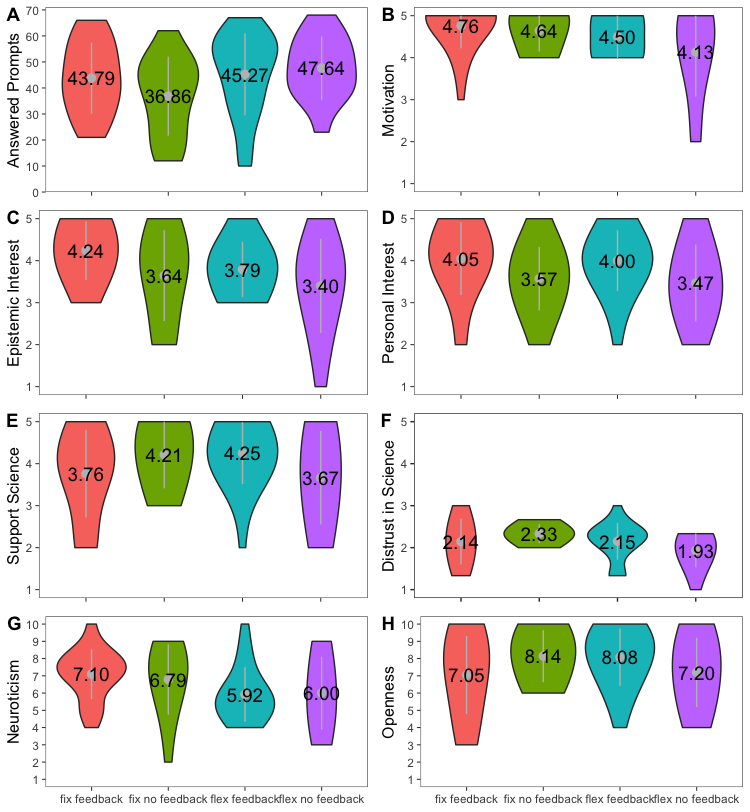
\includegraphics[width=\linewidth]{media/image1.png}


		\label{fig:rId35}
	\end{fullwidth}


	\end{figure*}









	\pagebreak

	\begin{table*}[t]
		\begin{fullwidth}
		
		
		\caption{ANOVA results for differences in participant motivation and sample characteristics in the incentivization scheme conditions.}
		\centering
		\begin{tabular}{@{} l l l l l l l l l l l l l l l l l l l l l l l l l l l l l l @{}}
			\hline \textbf{Outcome} & \multicolumn{3}{l}{\textbf{Payment}} & \multicolumn{3}{l}{\textbf{Feedback}}
			& \multicolumn{3}{l}{\textbf{Payment x Feedback}} \\

			  & F & p & η²\textsubscript{p} & F & p & η²\textsubscript{p} & F & p & η²\textsubscript{p}
			\\

			\hline Study Motivation & 5.96 & .017 & .078 & 2.36 & .129 & .033 & 0.61 &
			.436 & .009 \\

			  &  &  &  &  &  &  &  &  &  \\

			 Personal Interest & 0.16 & .695 & .002 & 6.80 & .011 & .089 & 0.02 & .883
			& .000 \\

			 Support Science & 0.02 & .893 & .000 & 0.09 & .768 & .001 & 5.50 & .022 &
			.073 \\

			 Financial Reasons & 0.00 & .949 & .000 & 0.05 & .819 & .001 & 2.50 & .118
			& .034 \\

			 Course Credit & 0.04 & .850 & .001 & 1.39 & .242 & .019 & 2.41 & .125 & .033
			\\

			 Fun & 1.47 & .229 & .021 & 0.89 & .349 & .013 & 2.47 & .121 & .034 \\

			 Epistemic Interest & 2.78 & .100 & .038 & 5.70 & .020 & .075 & 0.24 & .624
			& .003 \\

			  &  &  &  &  &  &  &  &  &  \\

			 Trust in Science & 3.53 & .065 & .048 & 0.02 & .889 & .000 & 3.90 & .052 &
			.053 \\

			 Interest in Science & 0.02 & .893 & .000 & 0.74 & .394 & .010 & 0.05 & .822
			& .001 \\

			 ATI & 0.04 & .838 & .001 & 0.41 & .524 & .006 & 0.05 & .823 & .001 \\

			  &  &  &  &  &  &  &  &  &  \\

			 Extraversion & 1.52 & .221 & .021 & 1.33 & .253 & .019 & 0.01 & .911 & .000
			\\

			 Agreeableness & 2.56 & .114 & .035 & 1.06 & .307 & .015 & 0.18 & .673 & .003
			\\

			 Conscientiousness & 0.83 & .366 & .012 & 0.74 & .394 & .010 & 0.93 & .339
			& .013 \\

			 Neuroticism & 5.50 & .022 & .073 & 0.07 & .788 & .001 & 0.22 & .641 & .003
			\\

			 Openness & 0.01 & .919 & .000 & 0.06 & .816 & .001 & 4.77 & .032 & .064 \\

			  &  &  &  &  &  &  &  &  &  \\

			 Age & 0.02 & .877 & .000 & .435 & .512 & .006 & .345 & .559 & .005 \\

			  &  &  &  &  &  &  &  &  &  \\

			 Overall Mood & 1.83 & .181 & .027 & 0.355 & .554 & .005 & 0.38 & .540 &
			.006 \\

			 Mean Mood & 0.00 & .976 & .000 & 0.589 & .446 & .009 & 0.14 & .710 & .002
			\\

			 SD Mood & 1.42 & .238 & .021 & 0.835 & .364 & .013 & 1.02 & .316 & .015
			\\

			  &  &  &  &  &  &  &  &  &  \\

			\hline  & Wald & P & OR & Wald & P & OR & Wald & P & OR \\

			\hline Gender & .261 & .609 & 1.43 & .537 & .464 & 1.67 & .005 & .905 & 0.91
			\\

			 Income & .339 & .560 & 1.36 & .611 & .434 & 1.51 & .056 & .812 & 1.29 \\


		\end{tabular}
	\end{fullwidth}
	\end{table*}




\end{document}